\documentclass[
    % english, % Klasei padavus parametrą 'english', darbas bus anglų kalba.
    % signatureplaces % prideda parašų vietas tituliniame puslapyje
]{VUMIFPSkursinis}
\usepackage{float}
\usepackage{wrapfig2}
\usepackage{hyperref}
\usepackage{algorithmicx}
\usepackage{algorithm}
\usepackage{algpseudocode}
\usepackage{amsfonts}
\usepackage{amsmath}
\usepackage{bm}
\usepackage{caption}
\usepackage{color}
\usepackage{graphicx}
\usepackage{listings}
\usepackage{subcaption}
\usepackage{biblatex}

% Titulinio aprašas
\university{Vilniaus universitetas}
\faculty{Matematikos ir informatikos fakultetas}
\department{Programų sistemų studijų programa}
\papertype{Kursinis darbas}
\title{Programų sistemų automatinių testų savaiminio atsistatymo mechanizmų analizė}
\titleineng{Evaluating Self-Healing Mechanisms in Software Test Automation}
\author{Vladimir Deriugin}
\status{4 kurso 2 grupės studentas}
% \secondauthor{Vardonis Pavardonis}   % Pridėti antrą autorių
\supervisor{prof. habil. dr. Dmitrij Nikolajev}
\reviewer{doc. dr. Vardenis Pavardenis}
\date{Vilnius – \the\year}

\bibliography{bibliografija}

\begin{document}
\maketitle

\tableofcontents

\section{Įvadas}

Pastaraisiais metais programinės įrangos kūrimo pramonė patiria reikšmingų pokyčių, kuriuos lemia sparčiai augantys reikalavimai kokybei ir produktų išleidimo greičiui. Agile ir DevOps metodologijos tapo pagrindiniais principais, užtikrinančiais kūrimo ir diegimo procesų lankstumą bei tęstinumą. Tokiomis sąlygomis testavimo automatizavimas įgauna esminę reikšmę, leidžiant kūrimo komandoms greitai aptikti ir ištaisyti klaidas, užtikrinant programinės sistemų stabilumą ir patikimumą. Tačiau dažni pokyčiai kode, sąsajoje ir infrastruktūroje, būdingi šiuolaikinėms kūrimo metodologijoms, sukelia nestabilumą testuose ir padidina jų palaikymo laiką. Dėl to aktuali tampa savaiminio atsistatymo mechanizmų įdiegimo tema programinės įrangos testavimo automatizavime.

\subsection{Temos aktualumas}

Šiuolaikinės kūrimo metodologijos, tokios kaip Agile ir DevOps, reikalauja nuolatinio testavimo ir diegimo, dažnai kasdien ar kas savaitę. Tai lemia dažnus pokyčius kodų bazėje, vartotojo sąsajoje (UI), DOM struktūroje ir API, kas savo ruožtu sukelia automatizuotų testų nestabilumą. Tradiciniai testų scenarijų palaikymo metodai tampa nepakankamai efektyvūs, nes reikalauja didelių laiko ir darbo išteklių testų pritaikymui prie pokyčių. Šiuo kontekstu savaiminio atsistatymo mechanizmai, naudojantys dirbtinį intelektą (DI) ir mašininį mokymą (MM), yra perspektyvus kryptis, galinti padidinti automatizuoto testavimo atsparumą ir efektyvumą.

Perėjimas prie išmanesnių testavimo sistemų yra lemiamas DI ir MM plėtros, leidžiančių savaiminio atsistatymo sistemoms tiksliau nustatyti gedimų priežastis ir automatiškai jas ištaisyti. Tai daro testavimo procesą atsparesnį ir sumažina priklausomybę nuo rankinio įsikišimo, kas savo ruožtu minimalizuoja laiką neveiklumo ir padidina testų scenarijų stabilumą. Tokių sistemų įdiegimas prisideda ne tik prie testavimo kokybės didinimo, bet ir prie laiko bei išteklių taupymo testų palaikyme.

\subsection{Tyrimo tikslas ir uždaviniai}

Pagrindinis šios kursinės darbo tikslas yra analizuoti savaiminio atsistatymo mechanizmų efektyvumą programinės įrangos testavimo automatizavime, siekiant nustatyti jų įtaką veikimo laiko sumažinimui ir testų scenarijų stabilumo padidinimui. Siekiant pasiekti nustatytą tikslą, reikia išspręsti šiuos uždavinius:

\begin{enumerate}
    \item Ištirti klaidų aptikimo ir taisymo būdus testuose, atsirandančius dėl pokyčių sąsajoje, DOM struktūroje, API ir kitose testuojamoje sistemoje elementuose.
    \item Atlikti savaiminio atsistatymo mechanizmų Testim ir Mabl platformose palyginimą, įvertinant jų tikslumą, atstatymo greitį ir klaidingų teigiamų rezultų skaičių.
    \item Įvertinti savaiminio atsistatymo mechanizmų poveikį testų scenarijų stabilumui ir palaikymui, taip pat laikui ir ištekliams, skiriamiems testų palaikymui, sumažinimui.
    \item Ištirti mašininio mokymosi integraciją į Testim ir Mabl savaiminio atsistatymo mechanizmus, įvertinant jų gebėjimą prisitaikyti prie naujų pokyčių ir klaidų tipų.
    \item Parengti rekomendacijas dėl platformų su savaiminio atsistatymo mechanizmais pasirinkimo ir naudojimo, siekiant padidinti automatizuoto testavimo efektyvumą.
\end{enumerate}

\subsection{Tyrimo objektas ir objektas}

Tyrimo objektas yra savaiminio atsistatymo mechanizmai automatizuotose programinės įrangos testavimo sistemose. Tyrimo objektas yra konkrečios šių mechanizmų įgyvendinimai Testim ir Mabl platformose. Testim ir Mabl yra šiuolaikiniai testavimo automatizavimo įrankiai, naudojantys DI ir MM prisitaikyti prie pokyčių testuojamuose taikomuose, minimizuojant rankinio įsikišimo poreikį ir didinant testavimo proceso bendrą patikimumą.

\subsection{Tyrimo metodai}

Siekiant tikslų ir išspręsti uždavinius šioje darbe bus naudojami šie tyrimo metodai:

\begin{enumerate}
    \item \textbf{Palyginamoji analizė}: Analizuoti Testim ir Mabl platformų funkcionalias galimybes ir savaiminio atsistatymo mechanizmus, įvertinant jų stipriąsias ir silpnąsias puses.
    \item \textbf{Eksperimentiniai tyrimai}: Vykdyti kontroliuojamus eksperimentus naudojant realius testavimo scenarijus ir taikymus, atlikti pokyčius testuojamame taikyme ir stebėti platformų elgesį atkuriant testus.
    \item \textbf{Veikimo ir metrikų analizė}: Rinkti ir analizuoti kiekybinius duomenis, susijusius su savaiminio atsistatymo mechanizmų veikimu, tokius kaip testų atkūrimo laikas, taisymų tikslumas ir klaidingų teigiamų rezultatų skaičius.
\end{enumerate}

\subsection{Darbo struktūra}

Kursinė darbas susideda iš aštuonių pagrindinių skyrių. Įvadas pagrindžia temos aktualumą, formuluoja tyrimo tikslus ir uždavinius, taip pat aprašo tyrimo objektą ir objektą, metodus bei darbo struktūrą. Antrame skyriuje pateikiamas literatūros apžvalga, apimanti pagrindines programinės įrangos testavimo automatizavimo sąvokas, savaiminio atsistatymo mechanizmus ir esamų sprendimų, įskaitant Testim ir Mabl, apžvalgą.

Trečiasis skyrius skirtas tyrimo metodologijai, aprašančiai metodų pasirinkimą, tiriamų platformų charakteristiką ir savaiminio atsistatymo mechanizmų efektyvumo vertinimo kriterijus. Ketvirtasis skyrius apima Testim ir Mabl analizę ir palyginimą, įskaitant funkcionalias galimybes, klaidų aptikimo ir taisymo metodus bei atliktų eksperimentų rezultatus.

Penkiasis skyrius aptaria gautus rezultatus, išryškindamas kiekvienos platformos privalumus ir trūkumus, taip pat jų įtaką testavimo procesams. Skyriuje „Išvados“ pateikiami pagrindiniai tyrimo rezultatai, pateikiamos rekomendacijos testavimo automatizavimo specialistams ir nagrinėjamos tolesnių tyrimų perspektyvos šioje srityje. Šeštasis skyrius apima literatūros sąrašą, o septintasis – prireikus, turi priedus su papildoma medžiaga.

\subsection{Teorinė bazė}

Analizuojant savaiminio atsistatymo mechanizmus programinės įrangos testavimo automatizavime, pagrindinė dėmesio dėmesio sutelkiama į šias teorines pagrindus ir koncepcijas:

\begin{enumerate}
    \item \textbf{Savaiminio atsistatymo sistemos (Self-Healing Systems)}:
    \begin{itemize}
        \item Savaiminio atsistatymo sistemų apibrėžimas ir veikimo principai.
        \item Savaiminio atsistatymo komponentai: gedimų aptikimas, priežasčių diagnostika, automatinis taisymas ir adaptacija.
    \end{itemize}
    
    \item \textbf{Programinės įrangos automatizuotas testavimas}:
    \begin{itemize}
        \item Pagrindinės testavimo automatizavimo metodologijos ir įrankiai.
        \item Testų scenarijų palaikymo ir priežiūros problemos taikyme ir jų sprendimo metodai.
    \end{itemize}
    
    \item \textbf{Mašininis mokymasis ir dirbtinis intelektas testavime}:
    \begin{itemize}
        \item Mašininio mokymosi algoritmų taikymas klaidų aptikimo ir taisymo tikslumo didinimui testuose.
        \item DI naudojimas sprendimų priėmimo automatizavimui, leidžiant prisitaikyti testus prie pokyčių be žmogaus įsikišimo.
    \end{itemize}
    
    \item \textbf{Nuolatinė integracija ir nuolatinis diegimas (CI/CD)}:
    \begin{itemize}
        \item Testavimo automatizavimo vaidmuo CI/CD srautuose.
        \item Savaiminio atsistatymo mechanizmų integracija į CI/CD procesus, siekiant užtikrinti testavimo sistemų stabilumą ir patikimumą.
    \end{itemize}
    
    \item \textbf{Metrikos ir efektyvumo vertinimas}:
    \begin{itemize}
        \item Pagrindiniai našumo rodikliai savaiminio atsistatymo mechanizmų efektyvumo vertinimui, tokie kaip atkūrimo laikas, taisymų tikslumas ir klaidingų teigiamų rezultatų sumažėjimas.
        \item Savaiminio atsistatymo mechanizmų diegimo įvertinimo kaštų ir naudos analizė testavimo automatizavimo procese.
    \end{itemize}
    
    \item \textbf{Automatizuoto testavimo įrankių palyginamasis analizė}:
    \begin{itemize}
        \item Palyginimo kriterijai: funkcionalios galimybės, adaptabilumas, našumas, integracija su kitais įrankiais.
        \item Pavyzdžiai remiantis Testim ir Mabl: detali savaiminio atsistatymo mechanizmų analizė ir palyginimas pasirinktuose įrankiuose.
    \end{itemize}
\end{enumerate}

\subsection{Praktinė reikšmė}

Atliktas tyrimas turi reikšmingą praktinę reikšmę, nes rezultatai gali būti naudojami programinės įrangos kūrėjams, testuotojams, kokybės užtikrinimo inžinieriams ir kokybės vadybininkams optimizuoti automatizuoto testavimo procesus. Efektyvių savaiminio atsistatymo mechanizmų įdiegimas leidžia sumažinti laiko ir išteklių sąnaudas testų palaikyme, padidinti jų patikimumą ir stabilumą, taip pat pagreitinti klaidų aptikimo ir taisymo procesą. Tai savo ruožtu prisideda prie galutinio produkto kokybės gerinimo ir įmonės konkurencingumo programinės įrangos rinkoje padidinimo.

\subsection{Tyrimo ribotumai}

Tyrimo metu gali kilti tam tikrų ribotumų, tokių kaip tiriamų platformų funkcionalių galimybių ribotumas, testuojamų taikymų ir scenarijų įvairovė, taip pat subjektyvumas vertinant kai kuriuos kokybinius rodiklius. Šie ribotumai gali turėti įtakos rezultatų apibendrinamumui ir reikalauja atsižvelgti į juos interpretuojant gautus duomenis.

\subsection{Išvados}

Taigi, tyrimas apie savaiminio atsistatymo mechanizmų efektyvumą programinės įrangos testavimo automatizavime yra aktualus ir reikalingas uždavinys šiuolaikinių sparčiai besivystančių technologijų ir kūrimo metodologijų sąlygomis. Tokių įrankių kaip Testim ir Mabl analizė leis nustatyti jų privalumus ir trūkumus, įvertinti jų indėlį į testų scenarijų stabilumo ir patikimumo didinimą, taip pat parengti rekomendacijas dėl jų efektyvaus naudojimo praktinėje veikloje. Šio tyrimo rezultatai gali prisidėti prie automatizuoto testavimo procesų optimizavimo, laiko ir išteklių sąnaudų sumažinimo, taip pat bendros kuriamos programinės įrangos kokybės padidinimo.

\section{Literatūros apžvalga}

\subsection{Programinės įrangos automatizuotas testavimas}
\subsection{Savaiminio atsistatymo mechanizmai}
\subsection{Esamų sprendimų apžvalga}
\subsection{Teorinės pagrindai}

\section{Tyrimo metodologija}

\subsection{Tyrimo metodų pasirinkimas}
\subsection{Testim ir Mabl platformų aprašymas}
\subsubsection{Testim}
\subsubsection{Mabl}
\subsection{Efektyvumo vertinimo kriterijai}
\subsection{Tyrimo vykdymo procedūra}

\section{Testim ir Mabl analizė ir palyginimas}

\subsection{Funkcionalios galimybės}
\subsubsection{Testim}
\subsubsection{Mabl}
\subsection{Savaiminio atsistatymo mechanizmų palyginamasis analizė}
\subsubsection{Palyginimas tarp Testim ir Mabl požiūrių klaidų aptikimui ir taisymui}
\subsubsection{Adaptacijos prie pokyčių taikyme analizė}
\subsection{Eksperimentų rezultatai}
\subsubsection{Gautų duomenų pateikimas (grafikai, lentelės)}
\subsubsection{Palyginamosios analizės rezultatų interpretacija}

\section{Rezultatų aptarimas}

\subsection{Duomenų interpretacija}
\subsection{Privalumai ir trūkumai}
\subsubsection{Testim stipriųjų ir silpnųjų pusių nustatymas atliktos analizės pagrindu}
\subsubsection{Mabl stipriųjų ir silpnųjų pusių nustatymas atliktos analizės pagrindu}
\subsection{Įtaka testavimo procesams}
\subsection{Tyrimo ribotumai}

\section{Išvados}

\subsection{Pagrindiniai išvados}
\subsection{Rekomendacijos}
\subsection{Tolesnių tyrimų perspektyvos}


\subsection{Poskyris}
Citavimo pavyzdžiai: cituojamas vienas šaltinis \cite{PvzStraipsnLt}; cituojami
keli šaltiniai \cite{Kavitha2022, PvzStraipsnLta, PvzKonfLt, PvzKonfEn, PvzKnygLt, PvzKnygEn,
PvzElPubLt, PvzElPubEn, PvzBakLt, PvzMagistrLt, PvzPhdEn}.
%Todo

\printbibliography  % Šaltinių sąraše nurodoma panaudota
% literatūra, kitokie šaltiniai. Abėcėlės tvarka išdėstomi darbe panaudotų
% (cituotų, perfrazuotų ar bent paminėtų) mokslo leidinių, kitokių publikacijų
% bibliografiniai aprašai. Šaltinių sąrašas spausdinamas iš naujo puslapio.
% Aprašai pateikiami netransliteruoti. Šaltinių sąraše negali būti tokių
% šaltinių, kurie nebuvo paminėti tekste (LaTeX tai sutvarko automatiškai).

% \sectionnonum{Sąvokų apibrėžimai}
\sectionnonum{Santrumpos}
Sąvokų apibrėžimai ir santrumpų sąrašas sudaromas tada, kai darbo tekste
vartojami specialūs paaiškinimo reikalaujantys terminai ir rečiau sutinkamos
santrumpos.

% Priedai
% Prieduose gali būti pateikiama pagalbinė, ypač darbo autoriaus savarankiškai
% parengta, medžiaga. Savarankiški priedai gali būti pateikiami ir
% kompaktiniame diske. Priedai taip pat numeruojami ir vadinami. Darbo tekstas
% su priedais susiejamas nuorodomis.
\appendix{Neuroninio tinklo struktūra}

\begin{figure}[H]
    \centering
    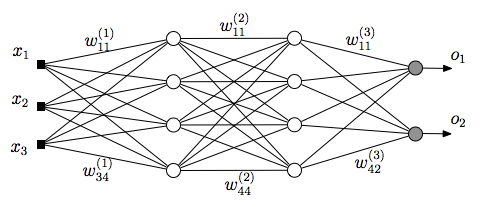
\includegraphics[scale=0.5]{img/MLP}
    \caption{Paveikslėlio pavyzdys}
    \label{img:mlp}
\end{figure}


\appendix{Eksperimentinio palyginimo rezultatai}

% tablesgenerator.com - converts calculators (e.g. excel) tables to LaTeX
\begin{table}[H]\footnotesize
  \centering
  \caption{Lentelės pavyzdys}
  {\begin{tabular}{|l|c|c|} \hline
    Algoritmas & $\bar{x}$ & $\sigma^{2}$ \\
    \hline
    Algoritmas A  & 1.6335    & 0.5584       \\
    Algoritmas B  & 1.7395    & 0.5647       \\
    \hline
  \end{tabular}}
  \label{tab:table example}
\end{table}

\end{document}
